\documentclass[10pt,a4paper]{labreport}
\usepackage{csquotes}
\usepackage{titlesec}
\usepackage{ragged2e}
\usepackage{siunitx}
\usepackage{setspace}
\usepackage{longtable}
\usepackage{rotating}
\usepackage{xurl}
\usepackage{physics}
\usepackage{caption}
\usepackage{wrapfig}
\usepackage{tabularray}
\usepackage{fancyhdr}
\usepackage{subcaption}
\usepackage{lscape}
\usepackage{tensor}
\usepackage{multirow}
\usepackage{chemformula}
\usepackage[gen]{eurosym}
\usepackage{float}
\usepackage{lipsum}
\usepackage{booktabs}
\usepackage{enumerate}
\usepackage[justification=justified]{caption}
\usepackage[nottoc]{tocbibind}
%  \usepackage[
% backend=biber,
% style=chem-acs,articletitle=true,doi=true]{biblatex}
% %\addbibresource{references.bib}





\title{Nanoscale Material Modelling
\\
\normalsize{Week 1}} % Main title and sub title. 

\author{Ilija A. Gjerapić, S4437586 i.a.gjerapic@student.rug.nl} % Name, student number, email

\supervisors{prof. dr. A. Giuntolli, prof. dr. J. Slawinski}

\begin{document}


\maketitle



  

\thispagestyle{firststyle}
\newpage
\section{Assignment 1}
\begin{enumerate}
  \item Visualize Quantum Espresso Simulations
  
  The visualization of the \texttt{Si.sci.in} input file is shown in Figure \ref{fig:ass1_cryst}. 
  \begin{figure}[h]
    \centering 
    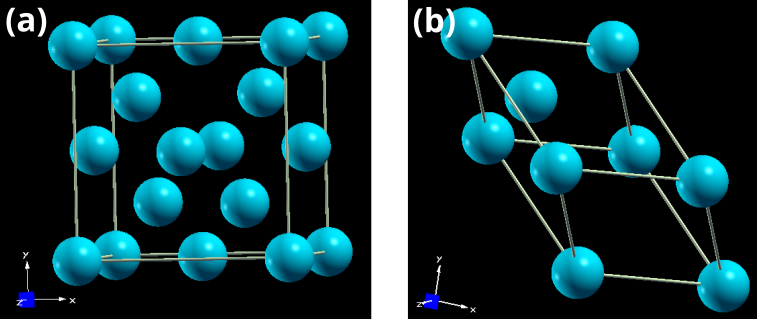
\includegraphics[width = 0.7\textwidth]{figs/ass1_Si_cryst.png}
    \caption{\textbf{(a)} The conventional FCC unit cell with a two atom basis. The lattice constant was found to be 5.43 \AA. (b) The primitive unit cell obtained from the input file. A lattice constant of 3.8396 {\AA} was found, with a bond angle of 60$^\circ$.}
    \label{fig:ass1_cryst}
  \end{figure}

  \item Visualize LAMMPS simulation 
  
  An overview of the total number of bonds and atoms can for each output file can be found in Table \ref{tab:ass1_lammps-bonds} and \ref{tab:ass1_lammps-atoms}, respectively.
  The types of atoms are clarified by considering a single isolated molecule in Figure \ref{fig:ass1_molecules}. Mainly, Type 1 corresponds to the backbone of the molecule, and Type 2 and 4 correspond to reactive atoms. Further analysis of the \texttt{half\_reacted.data} file showed that Type 3 atoms correspond to reacted Type 2 atoms, see Figure \ref{fig:ass1_molecules}. This reaction is also captured in the introduction of Type 2 bonds, as seen by the number of Type 2 bonds being exactly half of the number of Type 3 atoms. It is important to note, that this suggests that the Type 2 bond is restricted to two atoms. 

  \begin{table}[h]
    \caption{An overview of the number of each bond type for the output files considered.}
    \label{tab:ass1_lammps-bonds}
    \centering
    \begin{tabular}{cccc}
      \hline
    \textbf{Bond Type}      & \textbf{No-reacted}     & \textbf{Half-reacted}   & \textbf{Full-reacted}   \\
    \hline
    1 & 216000 & 216000 & 216000 \\
    2 & 0      & 10947  & 18861  \\
    3 & 0      & 0      & 0      \\
    4 & 0      & 0      & 0      \\ \hline
    \textbf{Total} & 216000 & 226947 & 234861 \\ \hline
    \end{tabular}
  \end{table}

  \begin{table}[h]
    \caption{An overview of the number of each atom type for the output files considered }
    \label{tab:ass1_lammps-atoms}
    \centering
    \begin{tabular}{cccc}
      \hline
    \textbf{Atom Type}      & \textbf{No-reacted}     & \textbf{Half-reacted}   & \textbf{Full-reacted}   \\
    \hline
    1 & 156000 & 156000 & 156000 \\
    2 & 48000  & 26106  & 10278  \\
    3 & 0      & 21894  & 37722  \\
    4 & 24000  & 24000  & 24000  \\ \hline
    \textbf{Total} & 228000 & 228000 & 228000 \\ \hline
    \end{tabular}
  \end{table}
  
  Using the \texttt{expression selection} feature in \texttt{Ovito} on the \texttt{no\_reaction.data} file, a single, non-bonded, molecule was found to be made up of 19 atoms. Further clustered-by-bonds analysis, Figure \ref{fig:cluster_analysis}, showed that the initial no-reaction configuration consisted of 12000 molecules. This also demonstrates that the system shows no polydispersity as 1200 $\times$ 19 gives the total number of atoms in the system. Similar clustering analysis on the half-reacted system revealed 1418 clusters with the largest consisting of 8123 molecules (154337) atoms while a single molecule was found for the full-reacted system provided by the \texttt{full\_reacted.data} file. 

  Instead of full molecules, the number of new chains formed by the reactions can be considered by first selecting the reacted atoms (Type 3) along with the atom connecting it to the main chain (Type 4) and then performing a similar cluster-by-bonds analysis, Figure \ref{fig:ass1_full_reaction}(a). 
  Such analysis reveals 6424 "clusters", with the largest consisting of 396 atoms. The distribution of the new chain sizes are shown in Figure \ref{fig:ass1_full_reaction}(b).

  \begin{figure}[htbp]
    \centering 
    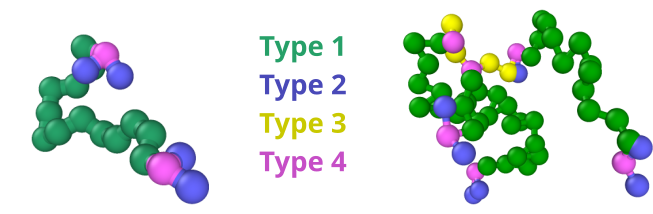
\includegraphics[width = 0.7\textwidth]{figs/ass1_molecules.png}
    \caption{Two isolated molecules demonstrated each atom type. The left shows an isolated molecule extracted from the non-reacted system, while the right was extracted from the half-reacted system.}
    \label{fig:ass1_molecules}
  \end{figure}
  \begin{figure}[htbp]
    \centering 
    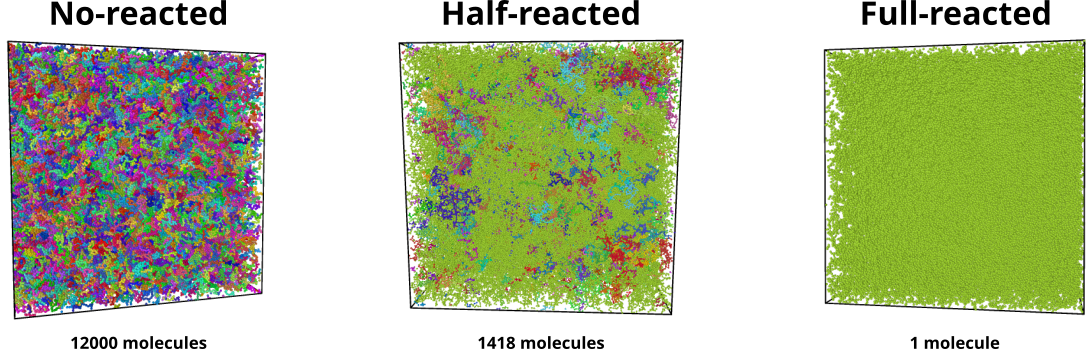
\includegraphics[width = 0.9\textwidth]{figs/ass1_molecule_clusters.png}
    \caption{Clusters of bonded atoms, considered molecules, as determined using \texttt{cluster by bonds} in \texttt{Ovito} on the different systems considered. Different colors represent a different molecule.}
    \label{fig:cluster_analysis}
  \end{figure}
  \begin{figure}[htbp]
    \centering 
    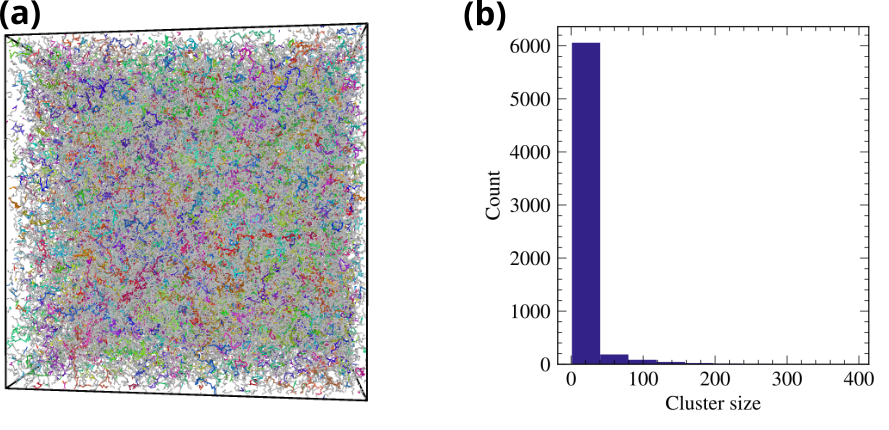
\includegraphics[width = 0.7\textwidth]{figs/ass1_full-reaciton.png}
    \caption{A cluster analysis by bonds for selecting atoms of Type 3 and Type 4. (a) Shows the different clusters (bonds only) with each color representing a separate cluster. (b) Shows the distribution of the cluster sizes using 10 bins. }
    \label{fig:ass1_full_reaction}
  \end{figure}
  
\end{enumerate}
\newpage
\section*{Assignment 2}
\begin{itemize}
  \item Energy Convergence
  \begin{itemize}
    \item From initial input, have a final total energy of \texttt{-20.43868608 Ry}. See convergence up to 10$^{-8}$ Ry after 7 iterations, which inline with our \texttt{conv\_thr} setting for the convergence threshold. Can increase accuracy by making a smaller convergence threshold. When doing so with \texttt{conv\_thr=1.0d-12} get same energy (up to 10$^{-8}$ Ry), but taking 10 iterations rather than seven with  \texttt{conv\_thr=1.0d-8}.
  \end{itemize}
  \item Very size of k-points mesh
  \begin{itemize}
    \item 
  \end{itemize}
  \item Vary size of kinetic energy cutoff
\end{itemize}




\section*{Assignment 3}

\section*{Assignment 4}



\newpage
% \printbibliography

% \begin{appendices}
%   \input{Appendix}
% \end{appendices}

\end{document}



